\chapter{Hardware Developed}
During the development of this thesis there was both hardware and software developed. In this chapter we are going to go through the hardware developed in order to build an appropriate \acrfull{soc} capable of running a full-fledged \acrfull{os}.

The \textit{IOb-SoC} was used as a \acrfull{soc} template. \textit{IOb-SoC} has some features that make it ideal to develop this project \acrshort{soc}. Firstly, it is open-source hardware. Witch means there are no royalties and the source code is publicly available. Secondly, adding new peripherals is very easy and intuitive, as it was previously seen in section \ref*{section:the_iob_soc_template}. Finally, it already has some features that make it ideal to use. \textit{IOb-SoC} already implements the interface with an internal (SRAM) and an external (DRAM) memory, contains iob-cache system and boot hardware unit. The boot hardware unit controls the first boot stage (also known as stage zero) that is executed after powering/resetting the system.

The hardware components that needed to be changed from \textit{IOb-SoC} were the \acrfull{cpu} and the \acrfull{uart} peripheral. The \acrshort{cpu} had to be changed because the previous \acrshort{cpu} (\textit{PicoRV32}) is not capable of running a full-feature \acrlong{os}. The \acrshort{uart} had to be swapped since there were no compatible Linux drivers that worked with \textit{iob-UART}. Besides swapping a few components from the chip new hardware had to be added. The additional hardware is the \acrshort{clint} and the \acrshort{plic} both compatible with RISC-V specifications. The \acrshort{clint} was added to implement timer and software interrupts on the \acrshort{soc}. The \acrshort{plic} was added to manage interrupts generated by other peripherals, for example from the \acrshort{uart}. A sketch of the \acrshort{soc} developed can be seen in figure \ref{fig:bd_linux}.

\begin{figure}[!h]
    \centering
    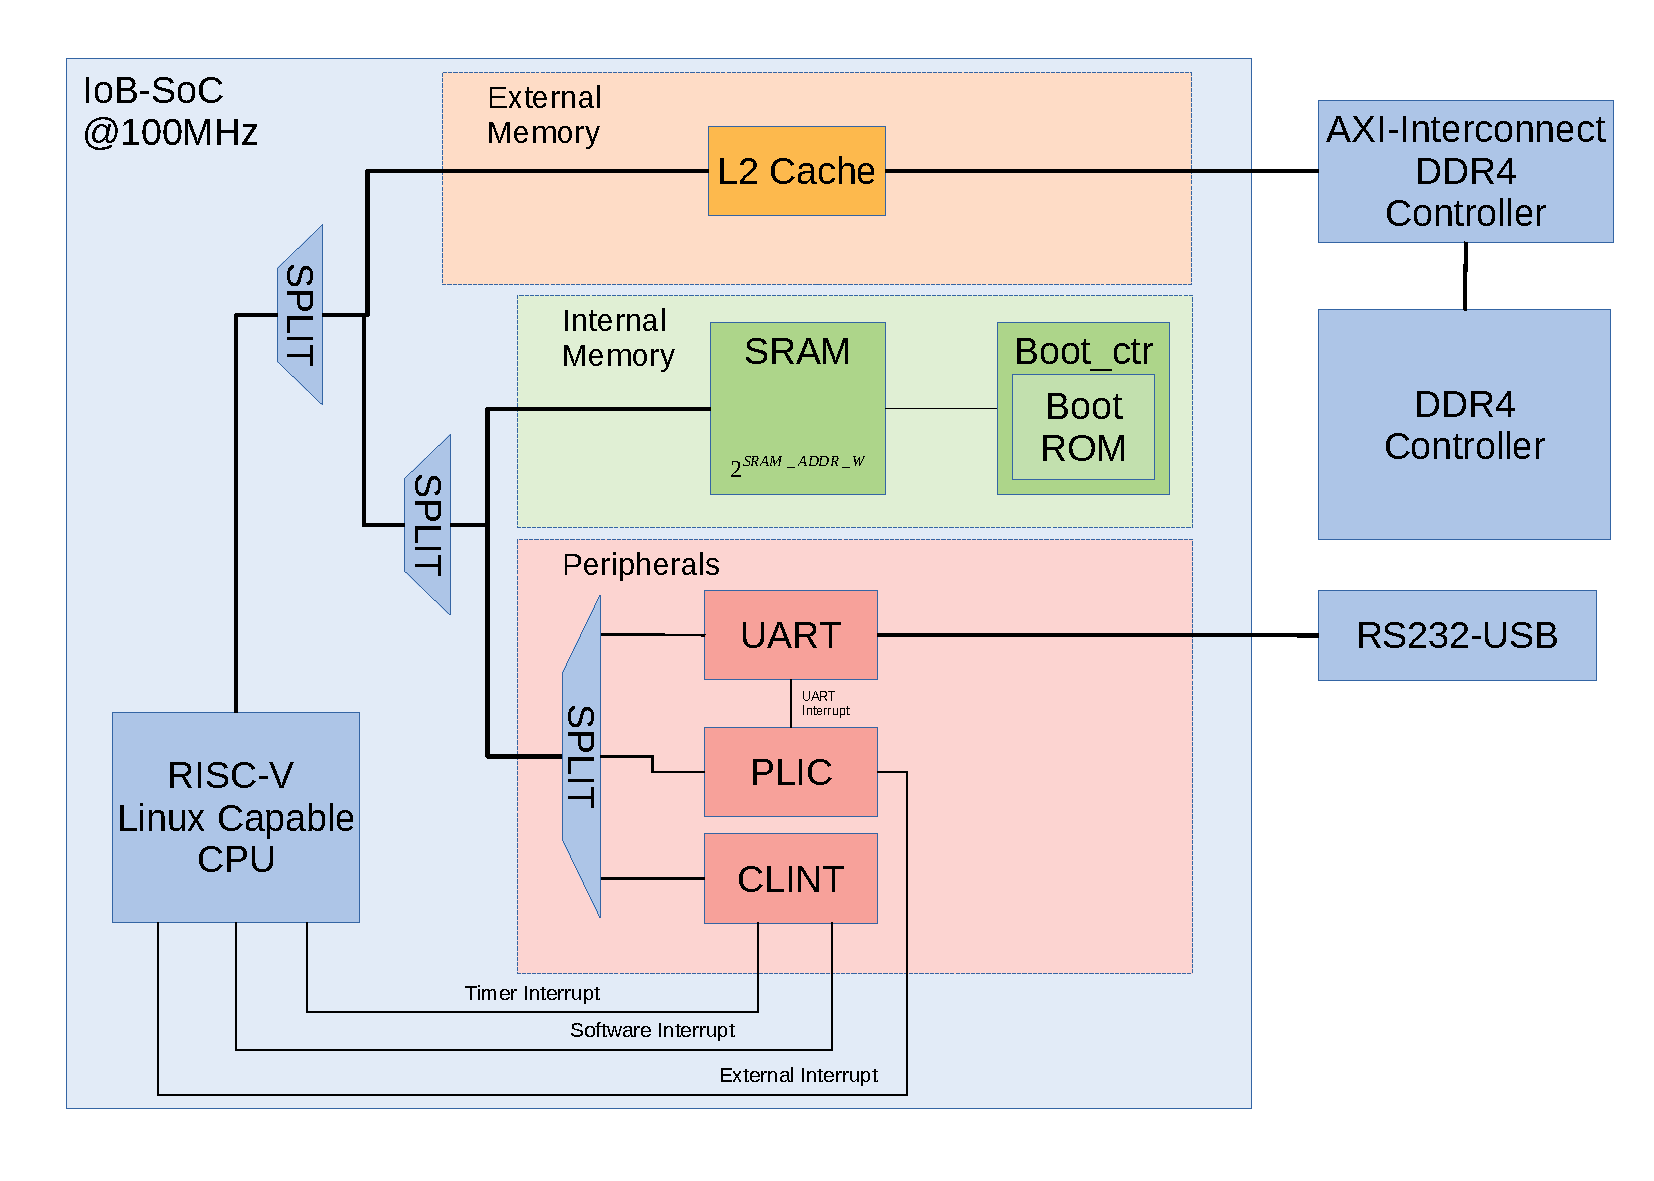
\includegraphics[width=0.7\linewidth]{bd_linux.pdf}
    \caption{Developed \acrshort{soc} sketch.}
    \label{fig:bd_linux}
\end{figure}

Comparing figure \ref{fig:bd_linux} with the original design of \textit{IOb-SoC} (figure \ref{fig:bd_original}) we can see that there were a few additional alterations. In the first place, it can be seen that the L1 Cache was removed. Since every application processor studied had a L1 cache built in, there was no need for the L1 \textit{iob-cache}. Next, a \textit{iob-split} was added to the \textit{IOb-SoC}. Previously, there was a single \textit{iob-split} for the data bus with three slaves (the internal memory, the external memory and the peripheral bus). This meant that there were 2 selection bits, when '00' then the internal memory bus was active, when '01' it was the peripheral bus and when '10' it was the external memory. This caused a problem because when addressing the external memory if its size is bigger than 1GB the selection bits would be '11'. The \acrfull{demux} output selected by '11' is not connected to anywhere, so this caused an internal hardware error. The solution was to include two \textit{iob-split} modules each one with two slaves. The first would chose between the external memory and either the internal memory or peripheral bus. The second would chose between the internal memory and the peripheral bus. Another advantage of using this method is that now the selection bits position does not vary depending on if we are using the DDR or not. This makes it easier to use external software that does not make use of the \textit{iob-soc} Makefiles. Before the peripheral addressing on external software had to be changed every time the developer wanted to test with or without the external memory.

During this project there was also an improvement on the \textit{IOb-SoC} verification. This lead to the creation of a top hardware module for the developed \acrlong{soc}.

\section{Central Processing Unit}
The \acrshort{cpu} chosen to use in this project was \textit{VexRiscv}. The performance of the CPU is not a significant issue for this project. However, how the core was designed and developed highly influenced the CPU decision. The flexibility of the CPU design, meaning how easily the CPU can be adapted to take advantage of the other components in \textit{IOb-SoC}, is an essential factor. Since the hardware and software developed in this project are open-source, the CPU implemented had to be open-source hardware. Moreover, knowing that the \textit{IOb-SoC} signals are 32-bit wide, ideally, the selected CPU should support RV32IMAC to facilitate its integration with IOb-SoC. From the \acrshort{cpu}s studied in chapter \ref{chapter:existing_embedded_technologies} \textit{VexRiscv} looked like the more indicated.

Generating the \acrshort{rtl} \textit{verilog} file from the \textit{SpinalHDL} hardware description is very simple. After cloning the \textit{VexRiscv} github repository the developer only has to run one command. Has it can be seen bellow in listing \ref{lst:rtl_vexriscv}. On the \textit{VexRiscv} repository there exist a couple of demo \acrshort{cpu} configurations. The configurations can be directly used or configured to generate a custom \textit{VexRiscv} core. There even already exists a demo configuration to generate a Linux compatible core. Although, in the developed hardware a custom core was implemented, the linux demo configuration was used as a starting point. Unfortunately, the Linux Demo design is outdated and the instructions, commented on the hardware configuration file, to run a Linux simulation and test the core do not work.

\begin{lstlisting}[language=make, caption={Generate \textit{verilog} from \textit{SpinalHDL}}, label=lst:rtl_vexriscv] 
git clone https://github.com/SpinalHDL/VexRiscv.git && \
  cd VexRiscv && sbt "runMain vexriscv.demo.LinuxGen"
\end{lstlisting}

The \textit{VexRiscv} can be configured by adding and removing plugins. Plugins are hardware components described in \textit{SpinalHDL} that can be reused in different designs by simply adding \enquote{\textcolor{green}{new} \textcolor{red}{Plugin\_Name}(...),} to the plugins list in the top \acrshort{cpu} description file. The existing plugins are described in the \textit{VexRiscv} repository on the \enquote{src/main/scala/vexriscv/plugin} directory. Looking at the available plugins it can be seen that there are two different plugins for the instruction bus and data bus each. They are \enquote{IBusSimplePlugin}, \enquote{IBusCachedPlugin}, \enquote{DBusSimplePlugin} and \enquote{DBusCachedPlugin}. The difference is that the cached plugins have the L1 Cache integrated, while on the simple plugins does not. An additional different between the data cached and simple plugin it that, although the \enquote{DBusCachedPlugin} fully supports the RISC-V atomic extension, the \enquote{DBusSimplePlugin} supports \acrfull{lr}/\acrfull{sc} but not \acrfull{amo} instructions. The \enquote{DBusSimplePlugin} could also be adapted to enable the full \enquote{A} extension, but since I do not understand how to code in \textit{SpinalHDL} it would be very time consuming.

The first step on implementing the \textit{VexRiscv} core on the \textit{IOb-SoC} was making sure that it worked on \enquote{bare metal} applications. Meaning it had to be working with the application accessing the silicon chip directly without any intermediary like an \acrfull{os}. This was done using the instruction and date simple plugins. The next step was to run the Linux kernel. To do so the instruction and data simple plugins had to be changed to the cached plugins. The missing support for \acrfull{amo} instructions was noticeable because the software would stop executing and enable an unknown instruction signal. It was possible to identify which instruction was causing the problem through the signal waves created during simulation.

The final \textit{VexRiscv} core configuration file contained the needed plugins to run a minimal \acrfull{os} based on Linux. The plugins present were:
% The file can be found in the project git hub repository under (\url{https://github.com/IObundle/iob-vexriscv/blob/cached_vexriscv/software/vexriscv_core/Linux.scala}).
\begin{itemize}
  \item The \enquote{IBusCachedPlugin} was added. With it the address of the first instruction the CPU had to fetch was defined by setting the reset value of the \acrfull{pc}. Also, it was specified that the CPU had no branch predictor and that it supported compressed instructions. The decision to not use any branch predictor was because there seemed to be a compatibility problem between the most recent RISC-V toolchain and the branch predictor that are available in the \textit{VexRiscv}. Since performance was not a concern in this project I choose to not use any branch predictor.
  \item The \enquote{DBusCachedPlugin} was added for the reason that it fully supported the atomic instructions.
  \item The \enquote{DecoderSimplePlugin} is used to decode the instructions.
  \item The \enquote{RegFilePlugin} implements the register file. This are the registers inside the CPU.
  \item The \enquote{IntAluPlugin} is used to calculate arithmetic and logic operations.
  \item The \enquote{SrcPlugin} is an auxiliary plugin for the plugins that contain \acrfull{alu}, Branch related hardware and Load/Store hardware logic.
  \item The \enquote{FullBarrelShifterPlugin} implements the shift instructions present in the RISC-V base \acrfull{isa}.
  \item The \enquote{HazardSimplePlugin} is used by the core to determine where it needs to stall.
  \item The \enquote{MulPlugin} allows the core to execute multiplication instructions.
  \item The \enquote{MulDivIterativePlugin} could be used to add multiplication and division support to the core (RISC-V M \acrshort{isa} extension). In this case it was used to add only division since the multiplication support was added by another plugin.
  \item The \enquote{CsrPlugin} is configured to fully support a Linux. This plugins adds the needed \acrfull{csr} to run a full feature \acrshort{os}. 
  \item The \enquote{DebugPlugin} was deactivated in the used core. But it could be used to debug the CPU core if there existed a JTAG interface. Currently the \textit{IOb-SoC} does not support it.
  \item The \enquote{BranchPlugin} allows the core to execute and make decisions on the jump instructions. This is part of the base \acrfull{isa}
  \item The \enquote{MmuPlugin} added support for the \acrfull{mmu}. Which is required to run a full feature \acrshort{os}.
  \item The \enquote{FpuPlugin} can add support for both the floats and doubles instruction extensions. In the core used this plugin was deactivated, since to run a minimal \acrshort{os} there is little to no advantage of using this extension. Causing the FPU to only be additional unnecessary hardware logic.
  %\item The \enquote{YamlPlugin} offers a service to other plugins to generate a useful Yaml file describing the CPU configuration. % It needs to be there for some reason. I donno.
\end{itemize}

After generating the verilog file that describes a \textit{VexRiscv} core I had to create a wrapper hardware module that adapted the \textit{VexRiscv} core interface to the \textit{IOb-SoC} internal bus.

\subsection{VexRiscv Wrapper}
The verilog wrapper, witch is called \textit{iob\_VexRiscv}, is instantiated by the \textit{IOb-SoC} top \acrshort{soc} hardware module as the \acrshort{cpu} component and instantiates the \textit{VexRiscv} core verilog module. The interface between the \textit{IOb-SoC} hardware and the \textit{VexRiscv} core is created by establishing a connection between the inputs and outputs from both sides.

The input signals of \textit{iob\_vexriscv} are: the clock signal which is the system clock derivative from the development board where the \acrshort{soc} is implemented; the reset signal which is set to high ('1') when the system reboots and when the stage 0 bootloader finishes; the boot signal that has the value '1' while the stage 0 bootloader is executing, after it finishes the boot signal value drops to '0' at the same time the reset signal is set to high; the instruction bus response signal that is connected to \enquote{cpu\_i\_resp}; the data bus response signal that is connected to \enquote{cpu\_d\_resp}; the timer interrupt and software interrupt signals which are set to '1' or '0' by the \acrshort{clint} unit; the external interrupt signal which is controlled by the \acrshort{plic} unit. The output signals are the instruction bus request signal and the data bus request signal, which connect to the \enquote{cpu\_i\_req} and \enquote{cpu\_d\_req} respectably. The \enquote{cpu\_i\_resp}, \enquote{cpu\_d\_resp}, \enquote{cpu\_i\_req} and \enquote{cpu\_d\_req} signals were reviewed in section \ref{section:the_iob_soc_template}. 

The input signals of the \textit{VexRiscv} core are: .... The output signals of the \textit{VexRiscv} core are: ....

After understanding the inputs and outputs of each module it is easy to see which wire should be connected to each other. But after connecting all the wires there were two problems. The fist being that the \textit{IOb-SoC} internal bus did not   contain all the signals that were needed by the \textit{VexRiscv} core. In order to successfully make the handshake with the \textit{VexRiscv} core an instruction and data request ready signal had to be generated. .... \textbf{How was it generated?}

\begin{table}[!h]
  \centering
  \begin{tabular}{ccc|c}
  valid\_reg & valid & resp\_ready & req\_ready \\ \hline
  0          & 0     & 0           & 0          \\
  0          & 0     & 1           & N/A        \\
  0          & 1     & 0           & 1          \\
  0          & 1     & 1           & N/A        \\
  1          & 0     & 0           & 0          \\
  1          & 0     & 1           & 1          \\
  1          & 1     & 0           & 0          \\
  1          & 1     & 1           & 1         
  \end{tabular}
  \caption{First try at identifying the rules the req\_ready should follow.}
  \label{tab:first_truth_table}
\end{table}

\begin{equation}
  (valid\_reg \cdot resp\_ready) + (valid \cdot \overline{valid\_reg} \cdot \overline{resp\_ready})
  \label{eq:first_logic_eq}
\end{equation}

\begin{table}[!ht]
  \centering
  \begin{tabular}{cc|c}
  valid\_reg & resp\_ready & req\_ready \\ \hline
  0          & 0           & 1          \\
  0          & 1           & N/A        \\
  1          & 0           & 0          \\
  1          & 1           & 1         
  \end{tabular}
  \caption{Simplified truth table.}
  \label{tab:simple_truth_table}
\end{table}

\begin{equation}
  (valid_reg \cdot resp_ready) + (\overline{valid_reg} \cdot \overline{resp_ready}) = valid_reg \odot resp_ready
  \label{eq:simple_logic_eq}
\end{equation}

The second problem was that after accepting an instruction or data request the values of the address, data and strb signals could change inside the \textit{VexRiscv} core. This changes would pass through \textit{iob\_VexRiscv} and reflect in the rest of \textit{IOb-SoC} hardware. Which caused the \textit{iob-cache} and peripherals to not function currently. This problem was solved by creating registers that saved the value of the address, data and strb signals when the request was accepted. The register values would then only change when the response was already received. 

To finalize, when the stage 0 bootloader was running the \acrfull{msb} of the instruction fetched address had to be forced to '0'. When defined that the firmware had to run from the external memory (RUN\_EXTMEM=1) the first instruction fetch should be at address $0x80000000$. To achieve this requirements the \acrfull{msb}, when RUN\_EXTMEM=1 was defined has the negated value of the boot signal, when RUN\_EXTMEM=0 it was forced to always be '0' since there is no need to access the external memory. On the data request bus it should also be taken into account that the \acrshort{msb} had to be '0' when the \acrshort{cpu} wanted to access the peripherals.

\section{UART16550 Wrapper}
The approach taken in this project was to adapt an existing open-source UART core that is supported by the Linux kernel. The other option was to create a Linux driver compatible with \textit{iob-UART} and compile the kernel with it. The chosen approach seamed more adequate and simpler solution.

\section{CLINT Unit}
\acrshort{clint}

\section{PLIC Unit Wrapper}
\acrshort{plic} 

\section{UUT Top Hardware}
This top module creates a \textit{verilog} wrapper of the \acrfull{uut} that allows it to interact with the different hardware logic simulators. The top module file is an adaptation of the previous \textit{verilog} file used on icarus simulation.

\begin{figure}[!ht]
    \centering
    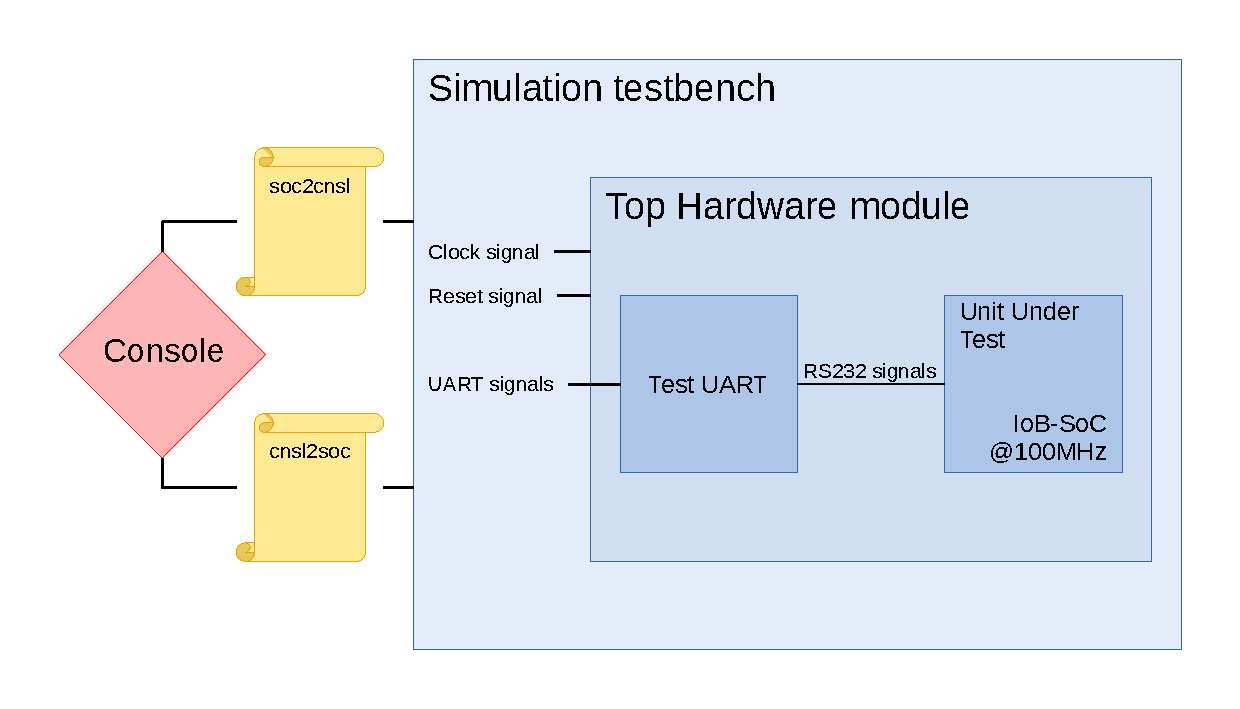
\includegraphics[width=\linewidth]{uut_top_hw.pdf}
    \caption{Simulated hardware interfaces.}
    \label{fig:uut_top_hw}
\end{figure}